\documentclass[12pt,a4paper]{article}
\usepackage[T2A]{fontenc}
\usepackage[utf8]{inputenc}
\usepackage[russian]{babel}
\usepackage{geometry}
\usepackage{tabularx} 
\geometry{margin=2.5cm}
\usepackage{amsmath,amssymb,mathtools}
\usepackage{enumitem}
\usepackage{tabularx}
\usepackage{hyperref}
\hypersetup{colorlinks=true,linkcolor=black,urlcolor=blue}
\setlength{\parindent}{0pt}
\setlength{\parskip}{6pt}
\begin{document}
{\Large\bfseries
\begin{flushleft}
Отчет по лабораторной работе №2 (Вариант №21)
\end{flushleft}}
\vspace{0.5em}\hrule\vspace{1.2em}

\section*{Задание}  
По имеющемуся академическому регулярному выражению построить:
\begin{itemize}
  \item минимальный ДКА, распознающий его язык (минимальность обосновать таблицей классов эквивалентности)
  \item возможно малый НКА, распознающий его язык. Возможно малый переключающийся (с конъюнкцией) КА, распознающий его язык. Частично обосновать таблицами множеств классов эквивалентности.
  \item расширенное регулярное выражение, распознающее тот же язык. В расширенном выражении можно использовать:
  \begin{itemize}
    \item wildcard-операцию \texttt{.} для замены произвольного символа алфавита;
    \item положительную итерацию $\tau^{+}$ и опцию $\tau?$. $\tau^{+} = \tau\tau^{*}$, $\tau? = (\tau|\varepsilon)$;
    \item операции предпросмотра $\tau_{0}(?= \tau_{1})\tau_{2} \equiv \tau_{0}((\tau_{1}.*)\cap\tau_{2})$ и ретроспективной проверки
          $\tau_{0}(?<= \tau_{1})\tau_{2} \equiv (\tau_{0}\cap(\tau_{1}.*))\tau_{2}$, а также их отрицательные версии
          $\tau_{0}(?! \tau_{1})\tau_{2} \equiv \tau_{0}((\tau_{1}.*)\cap\tau_{2})$ и
          $\tau_{0}?<! \tau_{1})\tau_{2} \equiv (\tau_{0}\cap(\tau_{1}.*))\tau_{2}$;
    \item классы букв $[c_{1} . . . c_{k}] \equiv (c_{1}|c_{2}|\ldots|c_{k})$ и их дополнения $[\char`^ c_{1} \ldots c_{k}]$.
    \item (обязательно) маркеры начала и конца выражения \^{} и \$.
  \end{itemize}
\end{itemize}

\section*{Исходное академическое регулярное выражение}
\[
((a|b)^{*}aa^{*}b(a|b)^{*}|bb^{*}a(a|b)^{*})abab(a|b)(a|b)
\]

\section*{Минимальный ДКА}
\begin{center}
\begin{minipage}{\linewidth}
\centering
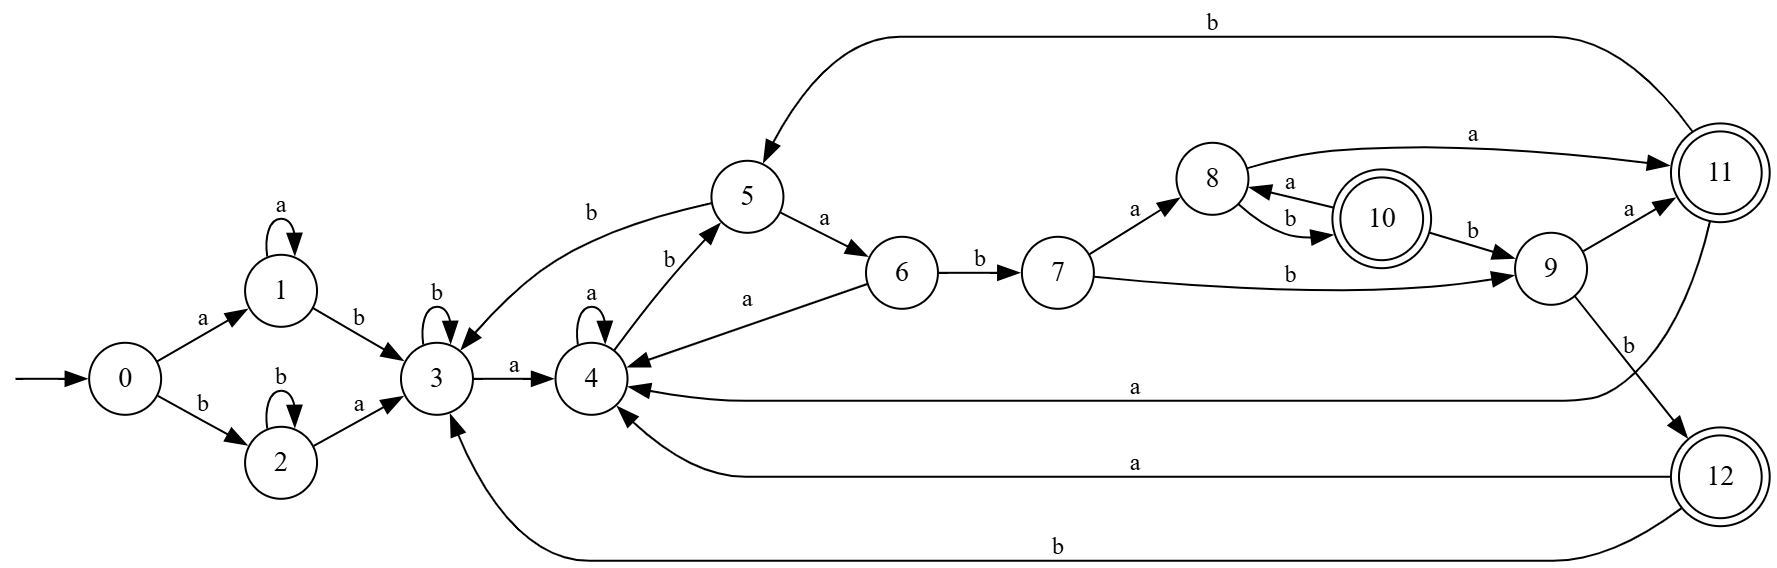
\includegraphics[width=1.0\linewidth]{mindfa.png}
\captionof{Рис. 1: Минимальный ДКА}
\label{fig:mindfa.png}
\end{minipage}
\end{center}

\textbf{Начальное состояние:} 0\\
\textbf{Финальные состояния:} 10, 11, 12\\
\textbf{Алфавит} $\Sigma=\{a,b\}$.

\begin{table}[ht]
\centering
\caption{Таблица переходов минимального ДКА}
\renewcommand{\arraystretch}{1.15}
\begin{tabular}{|c|c|c|}
\hline
\textbf{Состояние} & \textbf{a} & \textbf{b}\\
\hline
0  & 1  & 2   \\ \hline
1  & 1  & 3  \\ \hline
2  & 3  & 2  \\ \hline
3  & 4  & 3  \\ \hline
4  & 4  & 5  \\ \hline
5  & 6  & 3  \\ \hline
6  & 4  & 7  \\ \hline
7  & 8  & 9  \\ \hline
8  & 11  & 10  \\ \hline
9  & 11  & 12  \\ \hline
10 & 8  & 9  \\ \hline
11 & 4 & 5  \\ \hline
12 & 4 & 3  \\ \hline
\end{tabular}
\end{table}

\begin{table}[ht]
\vspace{-5pt}
\centering
\caption{Таблица классов эквивалентности}
\renewcommand{\arraystretch}{1.15}
\begin{tabular}{|c|c|c|c|c|c|c|c|c|c|c|}
\hline
\textbf{ } & $\boldsymbol{\varepsilon}$ & \textbf{a} & \textbf{aa} & \textbf{baa} & \textbf{abaa} & \textbf{babaa} & \textbf{ababaa} & \textbf{aababaa} & \textbf{bababaa} & \textbf{baababaa} \\
\hline
$\varepsilon$ & $-$ & $-$ & $-$ & $-$ & $-$ & $-$ & $-$ & $-$ & $-$ & $+$ \\ \hline
$a$           & $-$ & $-$ & $-$ & $-$ & $-$ & $-$ & $-$ & $-$ & $+$ & $+$ \\ \hline
$b$           & $-$ & $-$ & $-$ & $-$ & $-$ & $-$ & $-$ & $+$ & $-$ & $+$ \\ \hline
$ab$          & $-$ & $-$ & $-$ & $-$ & $-$ & $-$ & $+$ & $+$ & $+$ & $+$ \\ \hline
$aba$         & $-$ & $-$ & $-$ & $-$ & $-$ & $+$ & $+$ & $+$ & $+$ & $+$ \\ \hline
$abab$        & $-$ & $-$ & $-$ & $-$ & $+$ & $-$ & $+$ & $+$ & $+$ & $+$ \\ \hline
$ababa$       & $-$ & $-$ & $-$ & $+$ & $-$ & $+$ & $+$ & $+$ & $+$ & $+$ \\ \hline
$ababab$      & $-$ & $-$ & $+$ & $-$ & $+$ & $-$ & $+$ & $+$ & $+$ & $+$ \\ \hline
$abababa$     & $-$ & $+$ & $-$ & $+$ & $-$ & $+$ & $+$ & $+$ & $+$ & $+$ \\ \hline
$abababb$     & $-$ & $+$ & $-$ & $-$ & $-$ & $-$ & $+$ & $+$ & $+$ & $+$ \\ \hline
$abababab$    & $+$ & $-$ & $+$ & $-$ & $+$ & $-$ & $+$ & $+$ & $+$ & $+$ \\ \hline
$abababaa$    & $+$ & $-$ & $-$ & $-$ & $-$ & $+$ & $+$ & $+$ & $+$ & $+$ \\ \hline
$abababbb$    & $+$ & $-$ & $-$ & $-$ & $-$ & $-$ & $+$ & $+$ & $+$ & $+$ \\ \hline
\end{tabular}
\end{table}

Строки таблицы классов эквивалентности описывают состояния автомата и выступают в роли префиксов. Столбцы этой же таблицы выступают в роли суффиксов слов.\\
Все строки попарно различны, поэтому представленный автомат минимален


\newpage


\section*{Возможно малый НКА}
Для удобства построения НКА вместо исходного регулярного выражения 
\[
((a|b)^{*}aa^{*}b(a|b)^{*}|bb^{*}a(a|b)^{*})abab(a|b)(a|b)
\] 
я использую эквивалентное ему 
\[
(aa^{*}b|bb^{*}a)(a|b)^{*}abab(a|b)(a|b)
\]
Я могу утверждать, что они эквивалентны, поскольку отличаются только тем, как разбита на куски одна и та же «произвольная часть» слова, а не тем, какие именно слова описываются. Таким образом, оба выражения задают один и тот же язык. 

\begin{center}
\begin{minipage}{\linewidth}
\centering
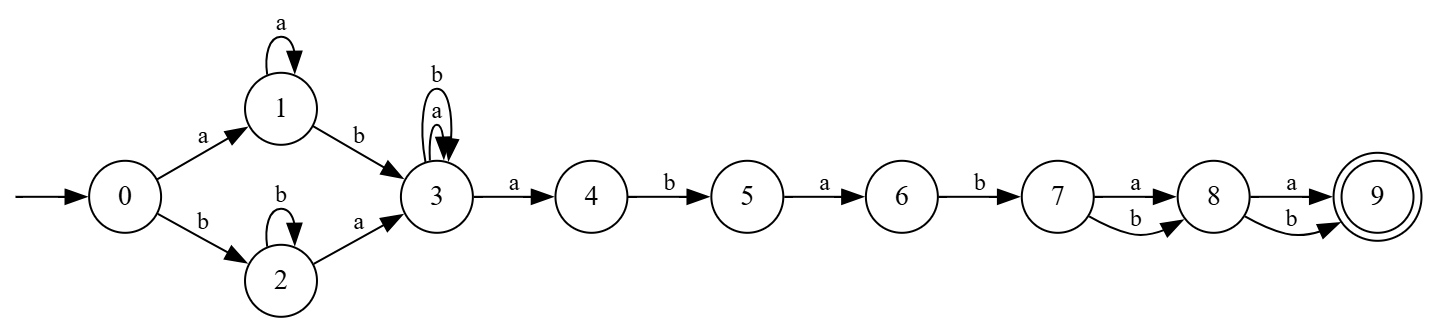
\includegraphics[width=1.0\linewidth]{posminnfa.png}
\captionof{Рис. 2: Возможно малый НКА}
\label{fig:posminnfa.png}
\end{minipage}
\end{center}

\textbf{Начальное состояние:} 0\\
\textbf{Финальное состояние:} 9\\
\textbf{Алфавит} $\Sigma=\{a,b\}$.

\begin{table}[ht]
\centering
\caption{Таблица переходов минимального ДКА}
\renewcommand{\arraystretch}{1.15}
\begin{tabular}{|c|c|c|}
\hline
\textbf{Состояние} & \textbf{a} & \textbf{b}\\
\hline
0  & 1  & 2   \\ \hline
1  & 1  & 3  \\ \hline
2  & 3  & 2  \\ \hline
3  & 3,4  & 3  \\ \hline
4  & -  & 5  \\ \hline
5  & 6  & -  \\ \hline
6  & -  & 7  \\ \hline
7  & 8  & 8  \\ \hline
8  & 9  & 9  \\ \hline
9  & -  & -  \\ \hline
\end{tabular}
\end{table}

\begin{table}[ht]
\centering
\caption{Таблица классов эквивалентности}
\renewcommand{\arraystretch}{1.15}
\begin{tabular}{|c|c|c|c|c|c|c|c|c|c|c|}
\hline
\textbf{ } & $\boldsymbol{\varepsilon}$ & \textbf{b} & \textbf{ab} & \textbf{bab} & \textbf{abab} & \textbf{babab} & \textbf{ababab} & \textbf{aababab} & \textbf{bababab} & \textbf{abababab} \\
\hline
$abababab$    & $+$ & $-$ & $+$ & $-$ & $+$ & $-$ & $+$ & $+$ & $+$ & $+$ \\ \hline
$abababa$     & $-$ & $+$ & $-$ & $+$ & $-$ & $+$ & $+$ & $+$ & $+$ & $+$ \\ \hline
$ababab$      & $-$ & $-$ & $+$ & $-$ & $+$ & $-$ & $+$ & $+$ & $+$ & $+$ \\ \hline
$ababa$       & $-$ & $-$ & $-$ & $+$ & $-$ & $+$ & $+$ & $+$ & $+$ & $+$ \\ \hline
$abab$        & $-$ & $-$ & $-$ & $-$ & $+$ & $-$ & $+$ & $+$ & $+$ & $+$ \\ \hline
$aba$         & $-$ & $-$ & $-$ & $-$ & $-$ & $+$ & $+$ & $+$ & $+$ & $+$ \\ \hline
$ab$          & $-$ & $-$ & $-$ & $-$ & $-$ & $-$ & $+$ & $+$ & $+$ & $+$ \\ \hline
$b$           & $-$ & $-$ & $-$ & $-$ & $-$ & $-$ & $-$ & $+$ & $-$ & $+$ \\ \hline
$a$           & $-$ & $-$ & $-$ & $-$ & $-$ & $-$ & $-$ & $-$ & $+$ & $+$ \\ \hline
$\varepsilon$ & $-$ & $-$ & $-$ & $-$ & $-$ & $-$ & $-$ & $-$ & $-$ & $+$\\ \hline
\end{tabular}
\end{table}

\newpage

Строки таблицы классов эквивалентности описывают состояния автомата и высту-
пают в роли префиксов. Столбцы этой же таблицы выступают в роли суффиксов
слов.\\
Главная диагональ таблицы состоит из плюсов, ниже нее находятся только минусы. Таким образом, таблица представляет собой нижне-трегуольную матрицу


\section*{Возможно малый переключающийся (с конъюнкцией) КА}
Представим построенный ПКА как пересечение двух регулярных языков:

\begin{enumerate}
  \item языка всех слов над алфавитом $\{a,b\}$, которые начинаются либо с блока «несколько букв $a$, затем буква $b$», либо с блока «несколько букв $b$, затем буква $a$»

  \item языка всех слов над алфавитом $\{a,b\}$, которые заканчиваются суффиксом вида $abab$ + две произвольные буквы из $\{a,b\}$».
\end{enumerate}

\begin{center}
\begin{minipage}{\linewidth}
\centering
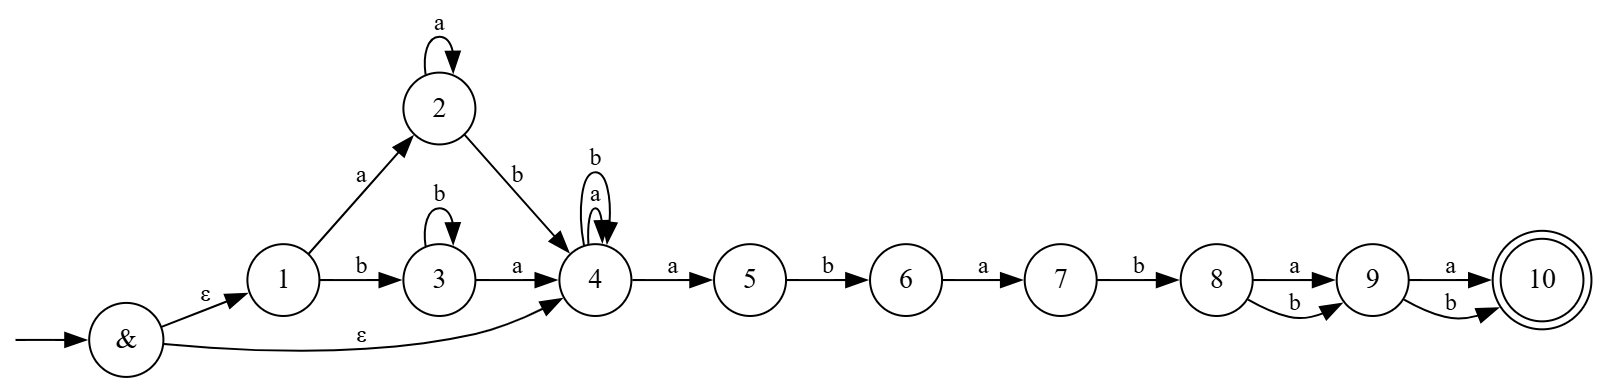
\includegraphics[width=1.0\linewidth]{posminafa.png}
\captionof{Рис. 3: Возможно малый ПКА}
\label{fig:posminafa.png}
\end{minipage}
\end{center}

\textbf{Начальное состояние:} $\&$\\
\textbf{Финальные состояния:} 10\\
\textbf{Алфавит} $\Sigma=\{a,b\}$.

\begin{table}[ht]
\centering
\caption{Таблица классов эквивалентности}
\renewcommand{\arraystretch}{1.15}
\begin{tabular}{|c|c|c|c|c|c|c|}
\hline
\textbf{ } & $\boldsymbol{\varepsilon}$ & \textbf{a} & \textbf{baa} & \textbf{babaa} & \textbf{ababaa} & \textbf{bababaa} \\ \hline
abababa & $-$ & $+$ & $+$ & $+$ & $+$ & $+$ \\ \hline
ababa   & $-$ & $-$ & $+$ & $+$ & $+$ & $+$ \\ \hline
aba     & $-$ & $-$ & $-$ & $+$ & $+$ & $+$ \\ \hline
ab      & $-$ & $-$ & $-$ & $-$ & $+$ & $+$ \\ \hline
a       & $-$ & $-$ & $-$ & $-$ & $-$ & $+$ \\ \hline
$\varepsilon$ & $-$ & $-$ & $-$ & $-$ & $-$ & $-$ \\ \hline
\end{tabular}
\end{table}

\newpage

Строки таблицы классов эквивалентности описывают состояния автомата и высту-
пают в роли префиксов. Столбцы этой же таблицы выступают в роли суффиксов
слов.
Главная диагональ таблицы состоит из минусов, выше нее находятся только плюсы.
Таким образом, таблица представляет собой верхне-трегуольную матрицу

\section*{Расширенное регулярное выражение}
В качестве исходного академического регулярного выражения выступает 
\[
((a|b)^{*}aa^{*}b(a|b)^{*}|bb^{*}a(a|b)^{*})abab(a|b)(a|b)
\]
Для построения расширенного регулярного выражения использую эквивалентное выражение, описывающее тот же язык: 
\[
(aa^{*}b|bb^{*}a)(a|b)^{*}abab(a|b)(a|b).
\]
Для построения расширенного варианта достаточно заменить конструкции вида $(aa^{*})$ и $(bb^{*})$ на положительную итерацию, то есть записать их как $(a^{+}b)$ и $(b^{+}a)$, а объединения вида $(a|b)$ и $(a|b)^{*}$ заменить на классы символов $[ab]$ и $[ab]^{*}$. Дополнительно используются маркеры начала и конца слова \verb!^! и \verb!$!, чтобы регулярное выражение описывало именно все слово целиком, а не произвольное вхождение внутри строки. В результате получаем расширенное регулярное выражение:

\begin{center}
\^{}$(a^{+}b|b^{+}a)[ab]^{*}abab[ab][ab]$\$
\end{center}

Можно усложнить запись за счёт явного использования wildcard-операции \texttt{.} и операции положительного предпросмотра, при этом сохраняется тот же язык. Основная идея состоит в том, чтобы заменить участок $[ab]^{*}$ на $.^{*}$, а две последние позиции $[ab][ab]$ на \texttt{..} . Таким образом можно описать «произвольную (в том числе пустую) последовательность символов» и «две произвольные буквы» с помощью wildcard-операции. Чтобы гарантировать, что все символы слова принадлежат алфавиту $\{a,b\}$, перед основным выражением добавляется положительный lookahead $(?=[ab]^{*}\$)$, который из начала строки проверяет, что вся строка целиком состоит только из $a$ и $b$. Таким образом, $.^{*}$ и \texttt{..} фактически ограничивается имеющимся алфавитом. Тогда запись расширенного регулярного выражения выглядит следующим образом:

\begin{center}
\^{}$(?=[ab]^{*}\$)(a^{+}b|b^{+}a).^{*}abab..$\$
\end{center}

Другие разрешённые в задании операции не использовались: для описания данного языка они не дают содержательных преимуществ и только усложняют запись.

\end{document}
